\documentclass{article}
\usepackage{amsmath, amssymb, amsthm}
\usepackage{fancyhdr}
\usepackage{lipsum} % for generating dummy text, you can remove this line in your actual document
\usepackage[margin=1in, bottom=1.5in]{geometry} % Adjust bottom margin as needed
\usepackage{thmtools}
\usepackage{listings}
\usepackage{graphicx}
\usepackage{hyperref}
\usepackage{esint}
\usepackage{circuitikz}

% Page style settings
\pagestyle{fancy}
\fancyhf{} % Clear header and footer
\renewcommand{\headrulewidth}{1pt}
\renewcommand{\footrulewidth}{1pt}
\renewcommand{\labelenumi}{(\alph{enumi})}
\fancyhead[C]{\textbf{\large 1A - Thermofluids}}
\fancyfoot[C]{\thepage}

\DeclareMathOperator{\tr}{Tr}

% Macros for convenience
\newcommand{\bbR}{\mathbb{R}} % Example: Real numbers
% Add more macros as needed

% Define theorems, propositions, definitions, etc. using thmtools
\usepackage{mdframed} % For framing
\declaretheoremstyle[
  spaceabove=6pt,
  spacebelow=6pt,
  headfont=\bfseries,
  notefont=\normalfont,
  bodyfont=\normalfont,
  headpunct={},
  postheadspace=1em,
  qed=,
]{mystyle}

\declaretheorem[
  style=mystyle,
  name=Example,
  within=section,
]{example}

% Define a framed theorem environment
\newmdtheoremenv[
  linecolor=black,
  linewidth=1pt,
  topline=true,
  bottomline=true,
  rightline=true,
  leftline=true,
  innertopmargin=10pt,
  innerbottommargin=10pt,
  innerrightmargin=10pt,
  innerleftmargin=10pt
]{proposition}{Proposition}

\newmdtheoremenv[
  linecolor=red,
  linewidth=1pt,
  topline=true,
  bottomline=true,
  rightline=true,
  leftline=true,
  innertopmargin=10pt,
  innerbottommargin=10pt,
  innerrightmargin=10pt,
  innerleftmargin=10pt
]{definition}{Definition}

\newmdtheoremenv[
  linecolor=red,
  linewidth=1pt,
  topline=true,
  bottomline=true,
  rightline=true,
  leftline=true,
  innertopmargin=10pt,
  innerbottommargin=10pt,
  innerrightmargin=10pt,
  innerleftmargin=10pt
]{theorem}{Theorem}

\begin{document}

\title{Engineering Tripos Part IA - Thermofluids}
\author{Morărescu Mihnea-Theodor}
\date{\today}

\maketitle

\newpage

\tableofcontents

\newpage

\section{Fluid Mechanics}

This part of the course is concerned with the mechanics of fluids. Our first question is: what exactly is a fluid? One might have seen before that a fluid is defined as a substance that is capable of flowing, i.e. taking the shape of the container it is in, however this is only partially correct.

\begin{definition}[Fluid]
    A fluid is a substance which, when at rest, cannot sustain shear stress.
\end{definition}

\subsection{Hydrostatics}

In this section of the course, we will first begin by analyzing the statics of fluids, also known as hydrostatics.

\begin{theorem}[Pascal's law]
    Pressure acts equally in all directions.
\end{theorem}

\begin{proof}
    To prove this theorem, we must first imagine an infinitesimally small right triangle on the surface of any object, of length $\Delta x$, height $\Delta z$, and width $b$ (into the page). Let $\Delta s$ be the length of the hypotenuse.

    By means of equilibrium, in the $x$ direction:

    \[ p_xb\Delta z - p_nb\Delta s \sin{\alpha} = 0\]

    In the $z$ direction, we deduce that in a similar fashion:

    \[ p_zb\Delta x - \frac{1}{2}\rho b \Delta x\Delta zg - p_nb\Delta s\cos{\alpha} = 0\]

    The geometry of the system yields us that $\sin{\alpha} = \frac{\Delta z}{\Delta s}$ and that $\cos{\alpha} = \frac{\Delta x}{\Delta s}$. By using this in the first equation, we obtain:

    \[ p_x = p_n \]

    In the second equation, this yields us:

    \[ p_z = p_n + \frac{1}{2}\rho g\Delta z \]

    However, this equation is unaffected by us varying $\Delta z$, and by our assumption that this is an infinitesimally small triangle, $\Delta z \to dz \to 0$, and thus:

    \[ p_z = p_n \]

    By combining our results, we obtain Pascal's law:

    \[ p_x = p_z = p_n \]
\end{proof}

\begin{proposition}[Hydrostatic pressure]
    The pressure in a fluid varies linearly, as given by:

    \[ p(z) = p_a + \rho gz \]

    Where $p_a$ is the atmospheric pressure, and $z$ is the depth below the free surface.
\end{proposition}

\begin{proof}
    By considering a small column of length $dz$, vertical equilibrium yields:

    \[ (p(z) + dp)A = (p(z) + \rho gdz)A \iff dp = \rho g dz \]

    Integrating this yields:

    \[ p(z) = p_0 + \rho gz \]

    Where $p_0$ is the pressure at $z = 0$, i.e. at the level of the free surface. Normally, we take this as $p_0 = p_a$, the atmospheric pressure.
\end{proof}

\subsubsection{Manometers}

The principles of hydrostatics are used to measure pressure using the U-tube manometer. A manometer is a U-tube device that is connected to two pressures, $p_A$ and $p_B$, with a column of air at both ends separating a column of liquid. We wish to determine the relationship governing the difference between the two aforementioned pressures.

Consider that the height between the levels of liquid on the left and right side is $h$. By applying hydrostatic pressure:

\[ p_2 = p_{\text{1, left}} + \rho_agh \]
\[ p_2 = p_{\text{1, right}} +\rho_lgh \]

We know that $p_2$ must be the same for both columns because of Pascal's law, however $p_1$ is different because we have two separate fluids (air and liquid). Now, we know that:

\[ p_{\text{1, left}} = p_A + \rho gz \]
\[ p_{\text{1, right}} = p_B + \rho gz \]

Since they are at the same height $z$. Therefore, we deduce the manometer equation:

\[ p_A - p_B = (\rho_l - \rho_a)gh \]

In the case where $\rho_l >> \rho_a$, this equation further degenerates into:

\[ p_A - p_B = \rho_lgh \]

\subsubsection{Barometers}

A mercury barometer is made from a long tube which is closed at one end and open at the other. It is filled with mercury and then inverted. As the vapour pressure of mercury is so low, we can ignore the pressure in the vacuum of mercury vapour which forms at the top. The height of the column simply indicates atmospheric pressure

At the free surface (where the barometer is put), the pressure is just $p_A$ - this is true for the lower end of the barometer. However, due to the height difference:

\[  p_A = p_v + \rho gh\]

Where $p_v$ is the pressure due to the mercury vapour forming on top. However, since $p_v << \rho gh$, we can assume that:

\[  p_A \approx \rho gh\]

\subsubsection{Archimedes' principle}

In the first section, we considered the triangular infinitesimally small element of surface from an object. Doing so again, and by considering equilibrium in the $z$ direction, we deduce that:

\[ p_zb\Delta x - p_nb\Delta s\cos{\alpha} - \frac{1}{2}\rho g b\Delta x\Delta z = 0 \]

The two pressures give rise to the upthrust, also known as the Archimedic force. By combining these two terms, we obtain:

\[ F_A = \rho gV \]

In other terms, the upthrust is equal to the weight of the displaced fluid.

\subsubsection{Forces on submerged bodies}

Consider that we want to determine the horizontal force acting on a rectangular strip which holds back stationary water. Therefore:

\[ F = \int_h^{h + w} \rho gwzdz = \rho g \left(h + \frac{w}{2}\right)w^2 \]

This is equal to the average force exerted on the wall, multiplied by the surface area. This concept can be further extended to a plane of width given by $b(s)$, inclined at an angle $\theta$, where $s$ is its current length:

\[ F = \int_S dF = \int \rho g s\sin{\theta}b(s)ds = \rho g \sin{\theta} \int sb(s)ds \]

Furthermore, to obtain the equivalent point of action of the force, we simply need to consider moment equilibrium:

\[ F\overline{s} = \int_S sdF \]

In general, for hydrostatic pressure distributions (and rectangular laminae), the equivalent point of action of the force is at:

\[ \overline{s} = \frac{2}{3}L \]

Where $L$ is the total length of the plane.

\newpage

\subsection{Fluid dynamics}

This section introduces the terminology of fluid dynamics required for proceeding with the course.

\begin{definition}[Streamline]
    A streamline is a curve in space which is always in line (parallel) to the velocity vectors at each point in the flow.
\end{definition}

Note that streamlines cannot cross each other (no mass can cross a boundary), as this would cause the flow two have two different velocity at one given instant. 

\begin{definition}[Stagnation point]
    Any object immersed in a flow has one or more stagnation points - these mark a point on the surface where the flow velocity is null.
\end{definition}

Note that in reality, an interesting effect can be seen - a particle never actually fully touches the boundary, as it would take $t \to \infty$ for that to happen.

\begin{definition}[Flow separation]
    Streamlines usually follow the surface of an object. However, flows will eventually separate from the surface when they cannot follow its curvature or if the pressure gradients become too large.
\end{definition}

\begin{definition}[Steady flow]
    We say that a flow is steady if the trajectories of particles passing through each point in space do not change with time. Conversely, we say that a flow is unsteady if it is not steady. Note that streamlines do not make sense in unsteady flow.
\end{definition}

\begin{definition}[Compressible flow]
    We say that a flow is compressible if the density is constant and uniform throughout the entire region. If, however, density is not constant, we say that the flow is incompressible.
\end{definition}

\begin{definition}[Viscosity]
    We say that a flow is viscous if it experiences viscous friction. This usually happens when the fluid is very close to the wall. Otherwise, we say that the flow is inviscid.
\end{definition}

Furthermore, the fluid infinitesimally close to the wall does not actually move (because of the interactions between particles) - this is also known as the no-slip condition. Viscous friction is characterised by the Reynolds number:

\[ Re = \frac{\rho v L}{\mu} \]

Where $\rho$ is the density of the fluid, $v$ is the velocity of the free stream (very far away), $l$ is a characteristic dimension, and $\mu$ is the viscosity.

\subsubsection{Systems and conservation principles}

\begin{definition}[Control volume/surface]
    A control volume is a region of space. A control surface is the surface of our choice of control volume.
\end{definition}

\begin{proposition}[Conservation of mass]
    The mass of a system must always remain constant, but the volume may change.
\end{proposition}

Suppose we have a control volume which has an inlet and an outlet. Therefore:

\[ m_t = \rho_0 V_0 + \rho_{\text{in}}A_{\text{in}}l_{\text{in}} \]
\[ m_{t + \Delta t} = \rho_0V_0 + \rho_{\text{out}}A_{\text{out}}l_{\text{out}} \]

Noting that $l = v\Delta t$ and by dividing both quantities by $\Delta t$:

\[ \rho_{\text{in}}A_{\text{in}}v_{\text{in}} = \rho_{\text{out}}A_{\text{out}}v_{\text{out}} \]

Equivalently:

\[ \dot{m_{\text{in}}} = \dot{m_{\text{out}}} \]

This is known as the continuity equation.

\begin{proposition}[Continuity]
    In steady flow, the continuity equation states that:

    \[ \oiint_{CS} \rho \textbf{v} \cdot \textbf{dA} = 0 \]

    This is equivalent to saying that the mass flow rate in equals the mass flow rate out. Note that we must always take the velocity component perpendicular to the area (this is why the scalar product is used).

    Equivalently, this can be stated as:

    \[ \sum_i \dot{m_i} = 0 \]

    Where $\dot{m_i} < 0$ for flow into a control volume (inlet), and $\dot{m_i} > 0$
    for flow outside of the control volume (outlet).
\end{proposition}

Note that the mass flow rate can be calculated using:

\[ \dot{m} = \int_A \rho \textbf{v} \cdot \textbf{dA} \]

\begin{proposition}[Conservation of momentum]
    Momentum is conserved in steady flow.
\end{proposition}

By Newton's second law, we deduce that:

\[ F = \frac{dp}{dt} = \frac{(mv)_{t + \Delta t} - (mv)_t}{\Delta t} = (\dot{m}v)_{\text{out}} - (\dot{m}v)_{\text{in}} \]

Where the quantity $\dot{m}v$ is also known as the momentum flow rate. The force $F$ acting on the fluid is given by all body forces (mechanical, electrostatic, electromagnetic etc.) and pressure forces. 

\begin{proposition}[Steady-flow momentum equation]
    Consider a steady flow problem. Then, we must have that:

    \[ \textbf{F} - \oiint_{CS} p\textbf{dA} = \oiint_{CS} \rho \textbf{v} (\textbf{v} \cdot \textbf{dA}) \]

    Otherwise, this can be stated as:

    \[ \sum F + \sum pA = \sum (\dot{m}v)_{\text{out}} - \sum (\dot{m}v)_{\text{in}} \]

    Notice that this relationship can be applied in any given direction in our control volume. Furthermore, the momentum flow rate can be calculated from:

    \[ (\dot{m}v) = \int_A \rho v (\textbf{v} \cdot \textbf{dA})  \]

    Note that $v$ must be the velocity component in the direction in which we are interested to apply equilibrium.
\end{proposition}

\newpage

\subsubsection{The equations of motion for fluid flow}

In this section, we will further analyze the behaviour of fluid elements under motion. Consider an infinitesimally small fluid particle (cubic) moving in a pressure gradient. Our goal is to find the force due to pressure in each direction.

\begin{figure}[h]
    \centering
    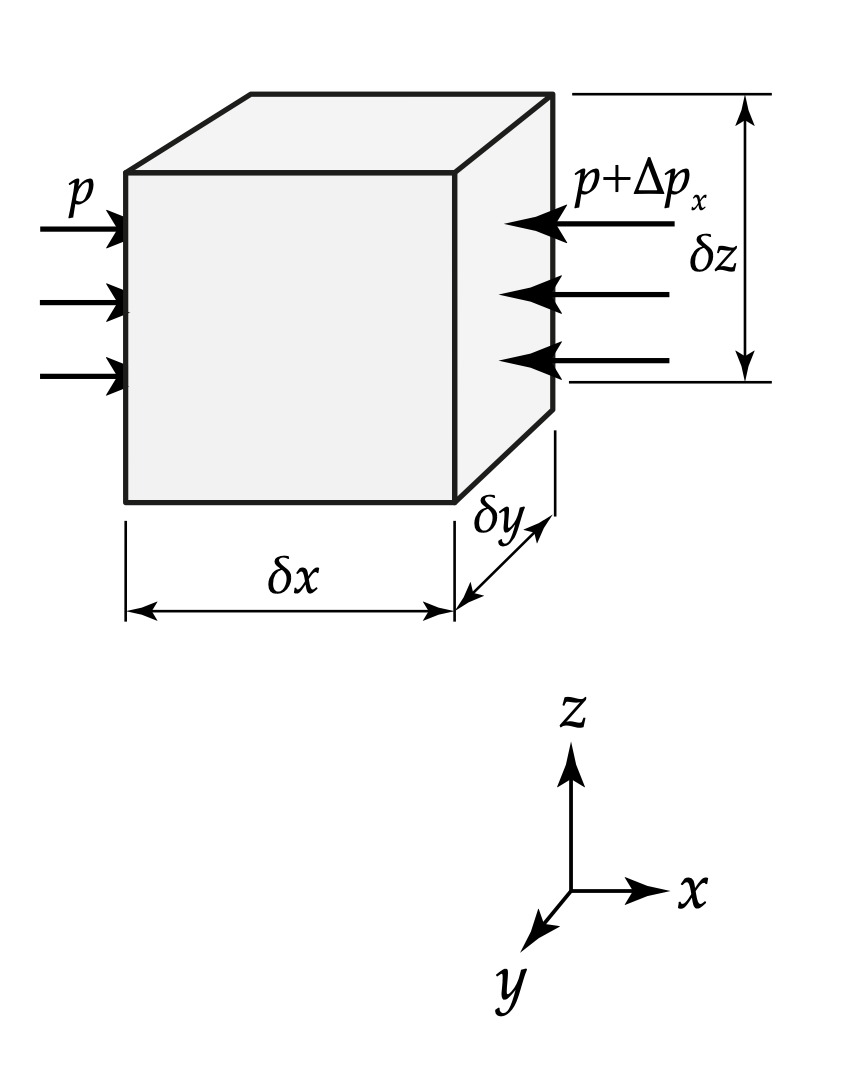
\includegraphics[width = 0.25\textwidth]{images/Screenshot 2024-02-20 at 17.32.41.png}
    \caption{Fluid element}
    \label{fig:enter-label}
\end{figure}

Since we are moving in a pressure gradient $\nabla p$, then the change in any direction is:

\[ \Delta p = \nabla p \cdot \mathbf{u} \]

Note that this is just the directional derivative. Let us now consider the $x$ direction. Therefore, the change of pressure is:

\[ \Delta p = \frac{\partial p}{\partial x} \delta x \]

By equilibrium (see figure):

\[ F = p\delta S - (p + \Delta p)\delta S \]

Because $\delta S = \delta y \delta z$, this can be expressed as:

\[ F = -\frac{\partial p}{\partial x}\delta x\delta y\delta z = -\frac{\partial p}{\partial x}\delta V \]

This is true for all directions. Therefore, we can further compress our relationship as:

\[ \mathbf{F} = -\nabla p \delta V \]

In other sources, this might appear as:

\[ \mathbf{a} = -\frac{1}{\rho}\nabla p \]

\begin{proposition}[Bernoulli's equation]
    Consider a steady flow problem. If there is negligible viscosity, no mixing/stagnation points, constant density, then along the streamline direction, at any two points:

    \[ p_1 + \rho g z_1 + \frac{1}{2}\rho v_1^2 = p_2 + \rho g z_2 + \frac{1}{2}\rho v_2^2 \]
\end{proposition}

\begin{proof}
    Consider a fluid particle (cubic, as before), and consider an intrinsic coordinate system $(s, n)$ moving along the fluid's path. Then:

    \[ \Ddot{s} = \frac{\partial v}{\partial t} = \frac{\partial s}{\partial t}\frac{\partial v}{\partial s} = v\frac{\partial v}{\partial s} \]

    Furthermore, as previously deduced, the force acting in the $s$ direction due to the pressure gradient is:

    \[ F_p = -\frac{\partial p}{\partial s}\delta V \]

    Lastly, the weight of the fluid particle is just:

    \[ W = -\rho \delta V g\frac{\partial z}{\partial s} \]

    By Newton's second law:

    \[ m\Ddot{s} = F_p + W \iff \rho \delta V v\frac{\partial v}{\partial s} = -\frac{\partial p}{\partial s}\delta V -\rho \delta V g\frac{\partial z}{\partial s} \]

    By dividing the above through $\delta V$ and rearranging, we deduce:

    \[ \frac{\partial p}{\partial s} + \rho g \frac{\partial z}{\partial s} + \rho v\frac{\partial v}{\partial s} = 0 \]

    Noting that $v\frac{\partial v}{\partial s} = \frac{1}{2} \frac{\partial }{\partial s}(v^2)$, we deduce that:

    \[ \frac{\partial}{\partial s}(p + \rho g z + \frac{1}{2}\rho v^2) = 0 \]

    This is equivalent to saying:

    \[ p + \rho g z + \frac{1}{2}\rho v^2 = \text{const} \]

    Thus, our proof is complete.
\end{proof}

Note that Bernoulli's equation is equivalent to the equation of motion of a fluid applied in the tangential $s$ direction. However, we still need to deduce the equation of motion in the normal direction.

\begin{proposition}[Normal equation of motion]
    Consider a steady flow problem. Then, the equation of motion for a region of fluid in the normal direction is:

    \[ \frac{\partial p}{\partial n} = \frac{\rho v^2}{R} \]

    Where $R$ is the radius of curvature of the streamline flow.
\end{proposition}

\begin{proof}
    Let us revisit the intrinsic $(s, n)$ coordinate system from mechanics.

    \begin{figure}[h]
        \centering
        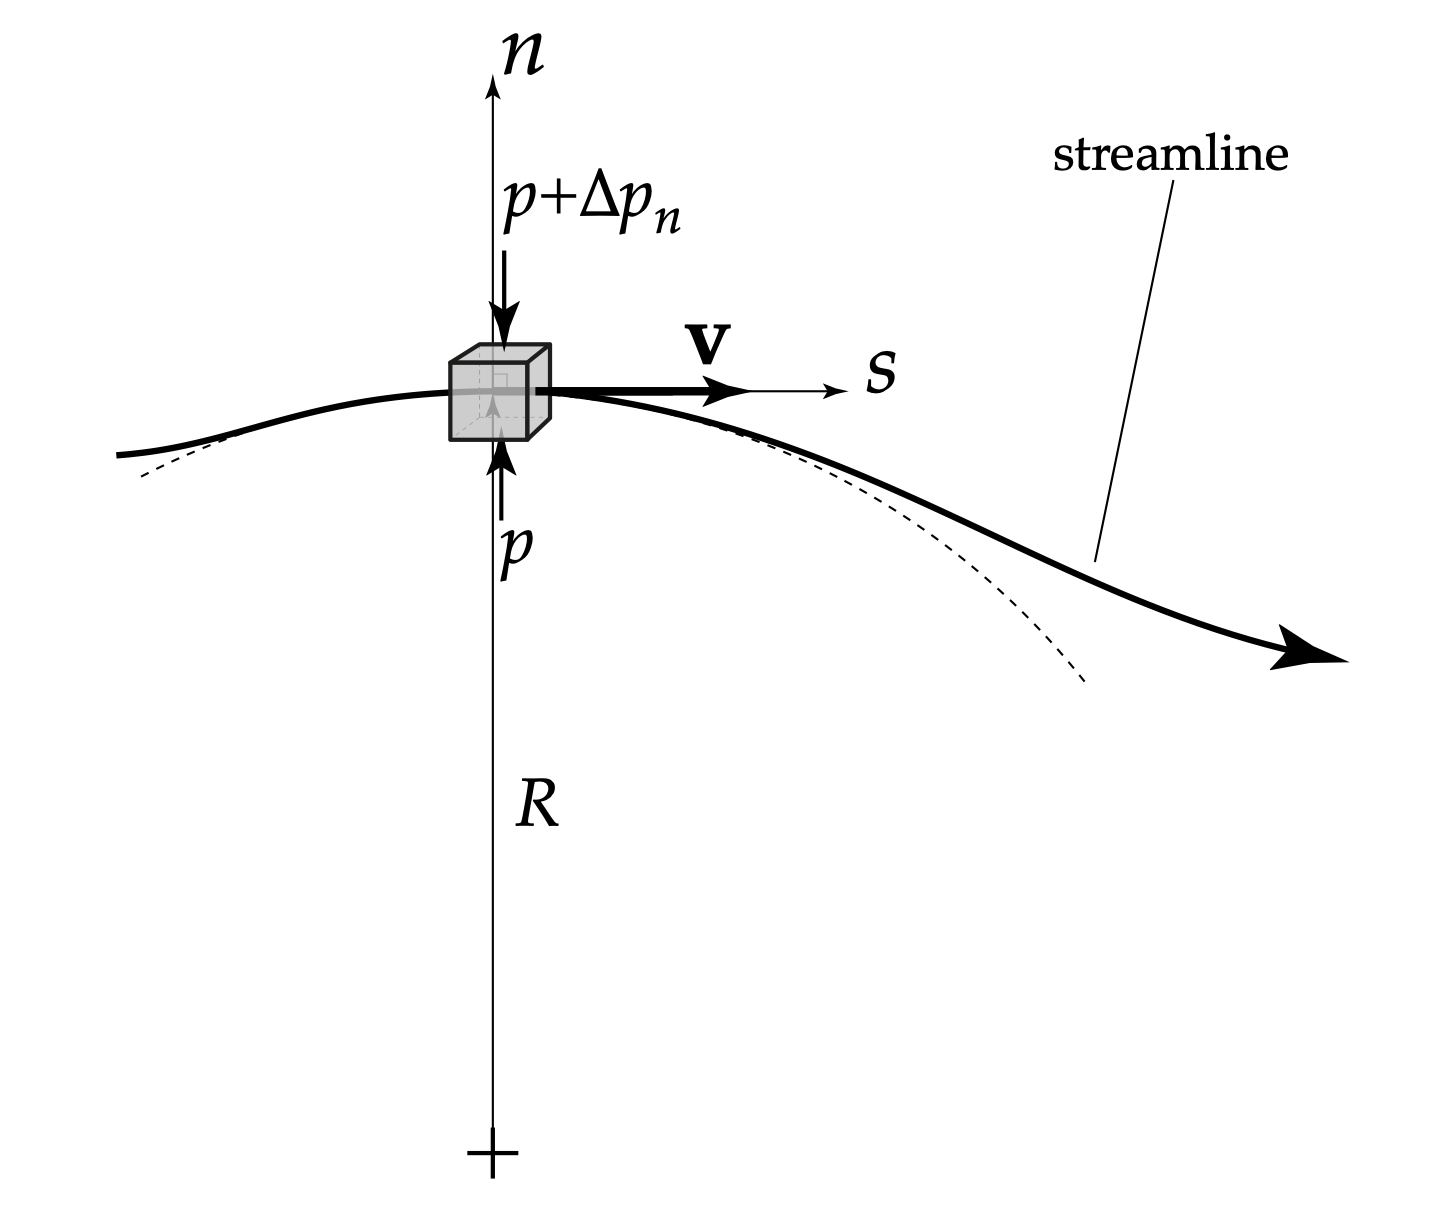
\includegraphics[width = 0.5\textwidth]{images/Screenshot 2024-02-20 at 17.53.25.png}
        \caption{Fluid particle}
        \label{fig:enter-label}
    \end{figure}

Because we are, again, considering a streamline, we must remember from the definition of a streamline that its velocity is only in the $s$ direction. Furthermore, form mechanics, the normal acceleration is:

\[ \Ddot{n} = \dot{s}\dot{\psi} = \frac{\dot{s^2}}{R} \]

Where $R$ is the radius of curvature. Note that in mechanics, $R$ is pointing towards the centre of curvature, whereas in fluid mechanics, we always choose $R$ to be pointing outwards. Hence, by the pressure gradient formula:

\[ -\frac{\partial p}{\partial n}\delta V = - \rho \delta V \frac{v^2}{R} \]

By dividing both sides by $\delta V$ (note that $m = \rho \delta V)$, we obtain:

\[ \frac{\partial p}{\partial n} = \rho \frac{v^2}{R} \]

Thus, our proof is concluded. Another important thing to note is that $\frac{\partial p}{\partial n} > 0$, since the right hand side of the equation is always positive. This means that if we go in the positive $n$ direction, pressure is always increasing, and if we go in the negative $n$ direction, pressure is decreasing. This is a fundamental result that allows us to explain many events we usually observe in nature, and other important effects, such as the Coandă effect.

\end{proof}

This result also allows us to explain why parallel flow has no pressure gradient. If we are in parallel flow, $R \to \infty$, and so, therefore:

\[ \frac{\partial p}{\partial n} \to 0 \]

Furthermore, it is important to note that in diverging flow, $\frac{\partial p}{\partial s} > 0$, and in converging flow, $\frac{\partial p}{\partial s} < 0$.

\begin{definition}[Coefficient of pressure]
    We define the pressure coefficient as:

    \[ C_p = \frac{p - p_\infty}{\frac{1}{2}\rho v_\infty^2} \]

    Note that the Bernoulli term $\frac{1}{2}\rho v_\infty^2$ is oftentimes called the dynamic pressure or dynamic head.
\end{definition}

\begin{proposition}[The Pitot-Static Tube]
    The Pitot-Static tube measures the difference between the pressure and the Pitot pressure. This can then be used to measure the velocity of the freestream flow. Consider a fluid path going from infinity (freestream), until the stagnation point. This yields:

    \[ p_\infty + \frac{1}{2}\rho v_\infty^2 = p_1 \]

    Since $v_1 = 0$, due to it being a stagnation point. Now, consider the second entrance:

    \[ p_\infty + \frac{1}{2}\rho v_\infty^2 = p_2 + \frac{1}{2}\rho v_\infty ^2 \]

    Because $v_2 = v_\infty$ (undisturbed flow). Hence, by combining the two equations:

    \[ p_1 = p_2 + \frac{1}{2}\rho v_\infty ^2 \]

    Yielding us:

    \[ v_\infty = \sqrt{\frac{2(p_1 - p_2)}{\rho}} \]
\end{proposition}

\begin{proposition}[The Coandă effect]
    Any jet of fluid sticks to a curved object's surface even after its curvature begins to decrease. This is explained by the streamline curvature equation:

    \[ \frac{\partial p}{\partial n} = \frac{\rho v^2}{R} \]

    Since this is always positive, we observe that because we traverse in the negative $n$ direction, the pressure must fall the closer we get to the surface. Therefore, $p_\infty$ is higher than the pressure at the surface of the object, leading to the fluid being pushed onto it, and sticking for longer than it should.
\end{proposition}

\begin{proposition}[The Magnus effect]
    If an object is rotated in a freestream flow, then the streamlines curve in a way which is similar to an aerofoil. Therefore, because of the streamline curvature equation, we expect lift to occur.
\end{proposition}

\newpage

\section{Thermodynamics}

\begin{definition}[Thermodynamic system]
    A thermodynamic system is an arbitrary geometrical portion of the universe with fixed or movable boundaries which may contain matter, energy, or both.

    We say that a thermodynamic system is closed if it represents a fixed quantity of matter, around which a boundary can be fixed. Everything inside the boundary is the system and everything outside is the surroundings (or the environment).

    Note that since no matter crosses the boundary, mass conservation is automatically satisfied for a closed system. Also note that energy can cross the boundary in the form of heat and work (which shall be defined later).
\end{definition}

\begin{definition}[Isolated system]
    We say that a (closed) system is isolated if there is no heat or work exchange between itself and its surroundings.
\end{definition}

\begin{definition}[Thermodynamic properties and state]
    A system possesses a number of thermodynamic properties, such as pressure, volume and temperature, which together define its thermodynamic state. Thermodynamic properties depend only on the state of the system, and not how the system arrived at that state.
\end{definition}

\begin{proposition}[Kelvin-Celsius relationship]
    Note that in Thermodynamics, we only work with absolute temperatures. Therefore:

    \[ T(K) = T(^\circ C) + 273.15 \]
\end{proposition}

\begin{definition}[Extensive property]
    We say that a property of a thermodynamic system is extensive if it depends on the size (extent) of the system. An example of this is the volume.
\end{definition}

\begin{definition}[Intensive property]
    We say that a property is intensive if it is not extensive. Typical examples include pressure and temperature.
\end{definition}

\begin{definition}[Specific property]
    We say that a property is specific if it is defined per unit mass. These are a subset of intensive properties.
\end{definition}

\begin{proposition}[The two property rule]
    For simple compressible systems at rest, two independent intensive properties and the mass are sufficient to fully define the state of the system, when it is in equilibrium. Thus:

    \[ p = p(T, V) \iff T = T(p, V) \iff V = V(p, T) \]
\end{proposition}

\begin{definition}[Thermodynamic equilibrium]
    A thermodynamic system is in equilibrium when none of its thermodynamic properties are changing in time at a measurable rate. Note that Thermodynamics can only furnish relationships connecting equilibrium states.

    However, if any process is carried out slowly, departures from equilibrium may be kept very small and the process effectively passes through a series of equilibrium states. This is referred to as a $\textbf{quasi-equilibrium}$ or $\textbf{quasi-static}$ process.
\end{definition}

\newpage

\subsection{The first law of Thermodynamics}

\begin{theorem}[The first law of Thermodynamics for closed systems]

Consider a closed system - it does not exchange matter with the surroundings (no mass crosses the  boundary), however, it may exchange energy in the form of either \textbf{heat} or \textbf{work}. Hence:

\[ \Delta E = Q - W \]

Where $\Delta E$ encapsulates kinetic, potential, and internal energy. If we neglect potential and kinetic energy terms, then:

\[ \Delta U = Q - W \]

In differential form, the statement of this law is:

\[ dU = \delta Q - \delta W \]
    
\end{theorem}

Note that heat and work are modes of energy transfer only, they do not reside in a system. Thus, they are not properties of any specific state.

\begin{proposition}[Resisted work]
    One type of work that we will frequently encounter is that due to a fully resisted expansion of a gas. Consider a system comprised of a gas held by a piston at a pressure $p$ on both sides. Then:

    \[ W = \int pdV \]
\end{proposition}

\begin{proof}
    The force acting on both sides of the piston is therefore $F = pS$. A small displacement $dx$ causes work to be done:

    \[ \delta W = Fdx \]

    Therefore:

    \[ W = \int Fdx = \int pSdx = \int pdV \]

    Note that this is only true in the case of a fully resisted transformation.
\end{proof}

\begin{definition}[Cyclic process]
    A cyclic process is one for which the system is returned to its original state. Because of this, in a cyclic process it is always true that:

    \[ \Delta U = 0 \]

    Furthermore, $\Delta U = Q - W \iff Q = W$ for the entire cycle. Hence:

    \[ Q = W = \oint pdV \]
\end{definition}

\begin{proposition}[The ideal gas equation of state]
    For many gases, experiments show that they obey the following relationship:

    \[ pV = n\overline{R}T \]

    This can be written as:

    \[ pV = mRT \text{   or   } pv = RT \]

    Where $R$ is the specific gas constant, $R = \frac{\overline{R}}{\mu}$, where $\mu$ is the molar mass of the gas.
\end{proposition}

Note that for a property $X$, we label $x$ as its specific equivalent, i.e.:

\[ x = \frac{X}{m} \]

This allows us to fully remove mass from the equation and only focus on the more important aspects of the problem. Also note that the specific volume $v = \frac{V}{m}$ is just the inverse density:

\[ v = \frac{1}{\rho} \]

\begin{definition}[Enthalpy]
    Consider a constant pressure process which is also fully resisted. Then:

    \[ W = \int pdV = p\Delta V \]

    The first law gives:

    \[ \Delta U = Q - W \iff Q = \Delta U + W \iff Q = \Delta U + p\Delta V \]

    This can then be written as:

    \[ Q = \Delta (U + pV) \]

    By defining $H := U + pV$ as the enthalpy of the system, then:

    \[ Q = \Delta H \]
\end{definition}

The units of enthalpy are the same as for energy, but note that enthalpy is \textbf{not} energy. It is merely just a short-hand for $U + pV$, and it is introduced because this combination appears very frequently.

\subsubsection{Specific heat capacities}

As we have previously seen, for a constant volume process, the first law gives:

\[ Q = \Delta U \]

And as previously, for a constant pressure process:

\[ Q = \Delta H \]

Accordingly, there must be two specific heat capacities, defined as follows:

\begin{enumerate}
    \item The constant volume (isochoric) specific heat capacity:
    \[ c_v = \left(\frac{\partial u}{\partial T}\right)_v \]
    \item The constant pressure (isobaric) specific heat capacity:
    \[ c_p = \left(\frac{\partial h}{\partial T}\right)_p \]
\end{enumerate}

Therefore, we can introduce the following definitions.

\begin{definition}[Ideal gas]
    A gas is said to be ideal if its internal energy $U = U(T)$ and enthalpy $H = H(T)$ are functions of temperature only.
\end{definition}

\begin{definition}[Semi-perfect gas]
    A gas is said to be semi-perfect if $c_v = c_v(T)$ and $c_p = c_p(T)$ are both functions of temperature.
\end{definition}

\begin{definition}[Perfect gas]
    A gas is said to be perfect if $c_v$ and $c_p$ are constants.
\end{definition}

\begin{definition}[Adiabatic exponent]
    We define the adiabatic exponent $\gamma$ of any gas as:

    \[ \gamma = \frac{c_p}{c_v} \]
\end{definition}

\begin{proposition}[The Robert-Mayer relationship]
    For any ideal gas, it is true that:

    \[ c_p = c_v + R \]
\end{proposition}

\begin{proof}
    We know from our definition that:

    \[ c_p = \left(\frac{\partial h}{\partial T}\right)_p = \left(\frac{\partial (u + pv)}{\partial T}\right)_p = \left(\frac{\partial u}{\partial T}\right)_p + \left(\frac{\partial (pv)}{\partial T}\right)_p\]

    Now, $pv = RT$, and therefore:

    \[ \left(\frac{\partial (pv)}{\partial T}\right)_p = R\]

    Because we have an ideal gas, the internal energy only depends on temperature, and then:

    \[ \left(\frac{\partial u}{\partial T}\right)_p = \left(\frac{\partial u}{\partial T}\right)_v = c_v \]

    Finally:

    \[ c_p = c_v + R \]
\end{proof}

\begin{proposition}
    For a perfect gas, by the above definitions, we have that:

    \[ du = c_vdT \text{   and   } dh = c_pdT \]
\end{proposition}

\subsubsection{Thermodynamic processes}

\begin{proposition}[The isobaric process]
    The isobaric process is a thermodynamic process which happens at constant pressure. Hence:

    \[ W = \int pdV = p\Delta V \]

    By applying the first law, $\Delta U = Q - W$, we obtain that:

    \[ Q = \Delta U + W = mc_v\Delta T + p\Delta V = mc_v\Delta T + mR\Delta T = mc_p\Delta T = \Delta H \]
\end{proposition}

\begin{proposition}[The isochoric process]
    The isochoric process is a thermodynamic process which happens at constant volume. Hence:

    \[ W = \int pdV = 0 \]

    Since $\Delta U = Q - W$, we obtain that the heat transfer is equal to the change in internal energy, i.e.:

    \[ Q = \Delta U = mc_v\Delta T \]
\end{proposition}

\begin{proposition}[The isothermal process]
    The isothermal process is a thermodynamic process which happens at constant temperature. Hence:

    \[ W = \int_A^B pdV = \int_A^B \frac{mRT}{V}dV = mRT \int_A^B \frac{1}{V}dV = mRT \ln{\frac{V_B}{V_A}} \]

    Because the temperature is constant, $\Delta U = mc_v\Delta T = 0$, and hence:

    \[ 0 = Q - W \iff Q = W \]
\end{proposition}

\begin{proposition}[The adiabatic process]
    The adiabatic process is a thermodynamic process in which there is no heat exchange. Let us start from the differential form of the first law:

    \[ dU = \delta Q - \delta W \]

    Since there is no heat exchange:

    \[ dU = -\delta W \iff m c_v dT = -pdV \iff m c_v dT + pdV = 0 \]

    Since $pV = mRT \iff p = \frac{mRT}{V}$, and so:

    \[ mc_vdT + \frac{mRT}{V}dV = 0 \iff c_v \frac{dT}{T} + R\frac{dV}{V} = 0 \]

    Noting that $\frac{R}{c_v} = \gamma - 1$, we obtain:

    \[ \frac{dT}{T} + (\gamma - 1) \frac{dV}{V} = 0 \iff \ln{\frac{T_2}{T_1}} + (\gamma - 1)\ln{\frac{V_2}{V_1}} = 0 \]

    Therefore:

    \[ \ln{\frac{T_2}{T_1}} = (\gamma - 1)\ln{\frac{V_1}{V_2}} \]

    And therefore, by exponentiating and multiplying:

    \[ T_1V_1^{\gamma - 1} = T_2V_2^{\gamma - 1} \iff TV^{\gamma - 1} = \text{const.} \]

    This equation can be manipulated into the two following forms:

    \[ pV^\gamma = \text{const.} \text{   or   } \frac{p}{T^{\frac{\gamma}{\gamma - 1}}} = \text{const.} \]
\end{proposition}

Beware of the assumptions involved in this process - it has to be adiabatic ($Q = 0$), the gas has to be perfect, and we have to be in quasi-equilibrium. This is also referred as the isentropic process.

\begin{proposition}[The polytropic process]
    The polytropic process is a thermodynamic process in which the pressure and volume are related by:

    \[ pV^n = \text{const.} \]

    Note that:

    \begin{enumerate}
        \item $n = \gamma$ represents an isentropic process
        \item $n = 1$ represents an isothermal process
        \item $n = 0$ is an isobaric process
        \item $n \to \infty$ is an isochoric process
    \end{enumerate}

    Furthermore, for $n \neq 1$, the work done is equal to:

    \[ W = \frac{p_1V_1 - p_2V_2}{n - 1} \]

    The first law can then be used to calculate the total heat transfer.
\end{proposition}

\newpage

\subsection{The second law of Thermodynamics}

The first law is the law of energy conservation - it makes no distinction between heat and work and only deals with their combined effect. However, the second law is the law of efficiency of energy conversion - it makes a great distinction between heat and work. We are now concerned with either irreversible processes (which take place in only one direction) and reversible processes (which can take place in either direction).

\begin{definition}[Irreversible process]
    In general, after a system undergoes an irreversible process, it can be restored to its initial state through suitable flows of heat and work from the surroundings. However, in doing so, the surroundings are changed permanently.

    The following types of processes are irreversible:

\begin{enumerate}
    \item Processes involving fluid friction of friction between solid surfaces
    \item Heat transfer across a finite temperature difference
    \item The unresisted or partially resisted expansion of a gas
    \item A rapid chemical reaction, such as an explosion
    \item The mixing of two different fluids
\end{enumerate}
\end{definition}

\begin{definition}[Reversible process]
    A process is said to be reversible if the system and its surroundings can be returned to ther initial state.
\end{definition}

Now, we will look at statements of the second law of thermodynamics. Both are statement of what cannot be achieved within a process.

\begin{theorem}[The Kelvin-Planck statement]
    It is impossible to construct a cyclic device whose sole effect is to produce positive work whilst receiving heat from a single thermal reservoir.
\end{theorem}

\begin{theorem}[The Clausius statement]
    It is impossible to construct a cyclic device whose sole effect is the transfer of heat from a cooler to a hotter body.
\end{theorem}

\subsubsection{Heat engines}

\begin{definition}[Thermal efficiency]
    The thermal efficiency of a cycle is defined as the net work done over the total heat input, i.e.:

    \[ \eta = \frac{W}{Q_H} = \frac{Q_H - Q_C}{Q_H} = 1 - \frac{Q_C}{Q_H} \]

    Therefore, using a Carnot cycle (two isothermal processes and two adiabatic processes), one can construct an engine with:

    \[ \eta = 1 - \frac{T_C}{T_H} \]
\end{definition}

\begin{theorem}
    The maximum efficiency of a cyclic heat engine operating between two thermal reservoirs is attained when the cycle is reversible.
\end{theorem}

\begin{theorem}
    All reversible heat engines operating between the same thermal reservoirs are equally efficient.
\end{theorem}

By the second theorem, because the Carnot cycle is reversible, the maximum efficiency we can obtain when oberating between two temperatures is the Carnot efficiency. Note that this also implies that:

\[ \frac{Q_H}{T_H} = \frac{Q_C}{T_C} \]

\subsubsection{Refrigerators and heat pumps}

Refrigerators and heat pumps are devices for extracting heat from a cold thermal reservoir and delivering (a greater quantity of) heat to a hotter thermal reservoir. Such devices do not violate the Clausius statement of the second law because they require a work input.

\begin{definition}
    For both of these, we define the coefficient of performance as:

    \begin{enumerate}
        \item For a refrigerator, COP$_R$ = $\frac{Q_C}{W}$
        \item For a heat pump, COP$_P$ = $\frac{Q_H}{W}$
    \end{enumerate}
\end{definition}

\newpage

\subsection{Thermal equilibrium and the zeroth law of Thermodynamics}

The following statement might be both trivial and obvious, but it is impossible to prove, and thus we need to take it as an axiom. Moreover, without it temperature cannot be defined.

\begin{theorem}[The zeroth law of Thermodynamics]
    If systems $B$ and $C$ are each separately in thermal equilibrium with system $A$, then they would be in thermal equilibrium with each other if brought into thermal contact.
\end{theorem}

Lord Kelvin created a temperature scale based on the second law, which is completely independent of any thermometric substance. The starting point is the fact that all reversible heat engines operating between the same two fixed temperatures have the same efficiency.

Consequently, for a heat engine:

\[ \frac{Q_1}{Q_2} = f(\theta_1, \theta_2) \]

On dimensional grounds:

\[ \frac{Q_1}{Q_2} = f\left(\frac{\theta_1}{\theta_2}\right) \]

The choice of this function is arbitrary, and the simplest form is used to define the thermodynamic temperature scale as:

\[ \frac{Q_1}{Q_2} = \frac{\theta_1}{\theta_2} = \frac{T_1}{T_2} \]

The equality between $\theta$ and $T$ follows from the previous section regarding heat engines. A single fixed point is required to define the size of the temperature unit (the Kelvin), and this is taken to be the triple point of pure water. This is the point at which ice, water and steam all coexist in equilibrium, and it is given the exact value of $0.01^\circ$C $ = 273.16$K on the thermodynamic scale.

\begin{theorem}[The Clausius inequality]
    The Clausius inequality states that:

    \[ \oint \frac{dQ}{T} \leq 0 \]

    This is the most concise mathematical statement of the second law.
\end{theorem}

This is a useful starting point for the next chapter of this course, where we will discuss entropy. Note that the convention is that $Q > 0$ if heat is transfered to the system, and $Q < 0$ when it is rejected. Also note that the inverse is true for work, i.e. $W < 0$ for work input and $W > 0$ fork work output.

\newpage

\subsection{Entropy}

Entropy is a property associated with the second law, just as energy is associated with the first law. In a previous chapter, we introduced the concept of irreversibility. It is therefore useful to have some means of quantifying the irreversibility that occurs during any process. This is achieved through entropy.

\begin{definition}[Entropy]
    The entropy of a system is an extensive thermodynamic property, defined as such:

    \[ dS = \left(\frac{dQ}{T}\right)_{\text{rev}} \]
\end{definition}

Note that if we wish to integrate the following and deduce the change in entropy, the integration must always be carried over a reversible path. Also note that if a process is reversible, then:

\[ dS = \frac{dQ}{T} \]

This shows that if a process is reversible and adiabatic, then it is also isentropic, i.e.:

\[ dS = 0 \]

\begin{proposition}[Equality of areas]
    Let us consider a cyclic reversible process. Then, the area under the $(p, V)$ diagram is equal to the area under the $(T, S)$ diagram.
\end{proposition}

\begin{proof}
    Note that because of the cycle being reversible, then $dS = \frac{dQ}{T} \iff dQ = TdS$. Then, by using the fact that we are within a cycle and the change in internal energy over the entire cycle is null:

    \[ \oint dQ = \oint dW \iff \oint TdS = \oint pdV \]
\end{proof}

\begin{proposition}[Entropy changes for an irreversible process]
    For an irreversible process, we have that:

    \[ dS \geq \frac{dQ}{T} \iff dS = \frac{dQ}{T} + dS_{\text{irrev}} \]
\end{proposition}

\subsubsection{Applications of entropy}

The entropy of a system cannot be measured directly, and so it must be inferred from the other properties, such as pressure, volume and temperature. 

\begin{proposition}[The entropy equations]
    Consider a simple compressible system undergoing an infinitesimal change of state by heat and work interactions with the surroundings. Therefore:

    \[ dU = \delta Q - \delta W \]

    If the process is reversible, then $dS = \frac{dQ}{T} \iff \delta Q = TdS$. Also, $\delta W = pdV$. Therefore:

    \[ dU = TdS - pdV \iff TdS = dU + pdV \]

    Noting that $dU = mc_vdT$ and that $pdV$ = $\frac{mRT}{V}dV$, we obtain:

    \[ TdS = mc_vdT + \frac{mRT}{V}dV \iff dS = \frac{mc_vdT}{T} + \frac{mR}{V}dV\]

    Taking the specific entropy of the system:

    \[ ds = c_v \frac{dT}{T} + R \frac{dv}{v} \]

    This can then be integrated to obtain the change of entropy in terms of temperature and volume. Furthermore:

    \[ H = U + pV \iff dH = dU + pdV + Vdp \]

    Noting that $TdS = dU + pdV$ from above:

    \[ dH = TdS + Vdp \iff TdS = dH - Vdp \]

    Therefore:

    \[ dS = mc_p\frac{dT}{T} - \frac{mR}{p}dp \]

    By taking the specific entropy:

    \[ ds = c_p \frac{dT}{T} - R\frac{dp}{p} \]

    This can then be integrated to obtain the change of entropy in terms of pressure and temperature.
\end{proposition}

Also note that any two of the words "adiabatic", "reversible" and "isentropic" imply the third. Also note that entropy is quantifiable through the Boltzmann relationship:

\[ S = k_B \ln{\Omega} \]

Where $k_B$ is the Boltzmann constant, and $\Omega$ is the number of microstates of the isolated system (what cannot be measured). However, we will only stick to the classical definition of entropy for the sake of practicality.

\newpage

\subsection{Reciprocating engines}

In this section, the theory developed so far is applied to analyse reciprocating engines, including petrol and diesel engines.

\subsubsection{The Stirling engine}

\begin{figure}[h]
    \centering
    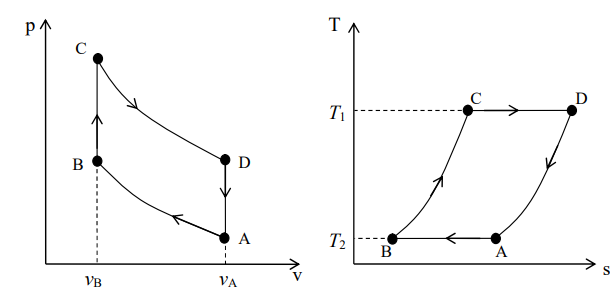
\includegraphics[width = 0.75\textwidth]{images/Screenshot 2024-04-03 165400.png}
    \caption{The Sirling engine cycle}
    \label{fig:enter-label}
\end{figure}

A Stirling engine is an example of a reciprocating external combusting engine - this is because the heat is transferred from an external source rather than by burning fuel internally, as is done within spark/compression ignition engines. A Stirling engine is comrpised of the following cycle:

\begin{enumerate}
    \item A $\to$ B: Isothermal compression at $T_2$
    \item B $\to$ C: Constant volume head addition
    \item C $\to$ D: Isothermal expansion at $T_1$
    \item D $\to$ A: Constant volume heat rejection
\end{enumerate}

Note that it can also be shown that the efficiency of a Stirling cycle is:

\[ \eta = 1 - \frac{T_2}{T_1} \]

Where $T_2 < T_1$ are the operating temperatures of the cycle.

\subsubsection{Spark \& compression ignition engines}

\begin{definition}[Spark ignition]
    A spark ignition engine is an engine (usually petrol engines) in which a mixture of air and vaporised fuel is introduced into the cylinder and ignited by a spark.
\end{definition}

\begin{definition}[Compression ignition]
    A compression ignition engine is an engine (usually diesel engines) in which air is compressed and reaches a high enough temperature that the fuel ignites spontaneously. The fuel is usually injected directly into the cylinder in the form of a liquid droplet spray.
\end{definition}

In general, a spark ignition engine functions in the following way:

\begin{enumerate}
    \item The induction stroke (A $\to$ B) - the inlet valve is opened and the piston moves downward, drawing the fuel-air mixture into the cylinder. The pressure falls below atmospheric pressure due to frictional losses in the intake system.
    \item The compression stroke (B $\to$ C) - both valves are closed and the piston moves upward compressing the mixture. The spark occurs before the top dead centre, and after a delay initiates rapid combustion at almost constant volume, causing a rapid increase in temperature and pressure.
    \item The power stroke (C $\to$ E) - the valves remain closed as the piston returns to the bottom dead centre. The pressure initially continues to rise as combustion is completed (D), and then falls as the hot gases expand. Work is done on the piston and transferred via the connecting rod to the crankshaft.
    \item The exhaust stroke (E $\to$ A) - the exhaust valve opens and the products of combustion are expelled as the piston returns to the top dead centre.
\end{enumerate}

\begin{figure}[h]
    \centering
    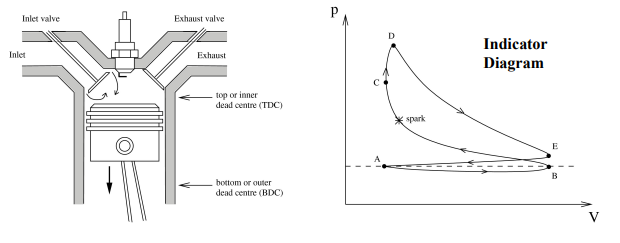
\includegraphics[width = \textwidth]{images/Screenshot 2024-04-03 170454.png}
    \caption{Spark ignition engine}
    \label{fig:enter-label}
\end{figure}

The compression ignition engine is very similar, except that instead of the spark, fuel is injected, and at a later stage. Combustion occurs more slowly, resulting in a flatter top to the indicator diagram.

\subsubsection{The air-standard cycles}

Air-standard cycles provide a very simplified model of the processes described above. The main approximations involved are:

\begin{enumerate}
    \item The working fluid is assumed to be air throughout, with constant specific heat capacities..
    \item The air is treated as a closed system and the combustion of the fuel is modelled as a heat addition from an external source.
    \item The compression and expansion processes are assumed to be adiabatic and reversible, thus isentropic. Note that heat losses may be significant in reality, especially during the power stroke.
\end{enumerate}

\begin{proposition}[The air-standard Otto cycle]
    The Otto cycle provides an approximate model of spark ignition engines and comprises the following four processes:

    \begin{enumerate}
        \item A $\to$ B: Isentropic compression
        \item B $\to$ C: Heat addition at constant volume
        \item C $\to$ D: Isentropic expansion
        \item D $\to$ A: Heat rejection at constant volume
    \end{enumerate}

\end{proposition}

\begin{figure}[h]
        \centering
        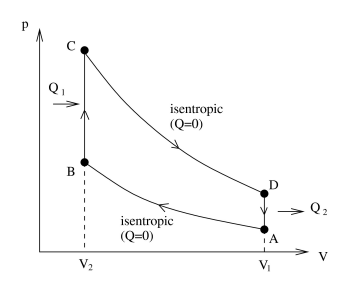
\includegraphics[width = 0.5\textwidth]{images/Screenshot 2024-04-03 171044.png}
        \caption{The Otto cycle}
        \label{fig:enter-label}
    \end{figure}

Note that in a real engine, the final process replaces expulsion of the exhaust gas and renewal with fresh charge in the real engine. Also, the ratio between the maximum and minimum volume is called the compression ratio, $r_v = \frac{V_1}{V_2}$.

This gives us the following efficiency for the Otto cycle:

\[ \eta = 1 - \frac{1}{r_v^{\gamma - 1}} \]

\begin{proposition}[The air-standard Diesel cycle]
    The Diesel cycle provides an approximate model of compression ignition engines, and comprises the following four processes:

    \begin{enumerate}
        \item A $\to$ B: Isentropic compression
        \item B $\to$ C: Heat addition at constant pressure
        \item C $\to$ D: Isentropic expansion
        \item D $\to$ A: Heat rejection at constant volume
    \end{enumerate}
    
\end{proposition}

Note the similarities between the two engines - only one process differs. Also, the constant pressure heat addition is intended to model the slower combustion process. As before, we define the same compression ratio, and also the cut-off ratio:

\[ \alpha = \frac{V_3}{V_2} \]

\begin{figure}[h]
    \centering
    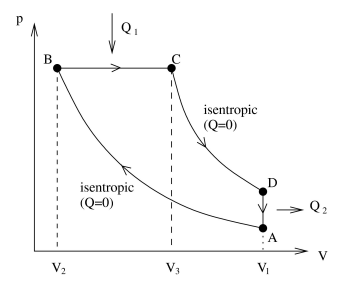
\includegraphics[width = 0.5\textwidth]{images/Screenshot 2024-04-03 171618.png}
    \caption{The Diesel cycle}
    \label{fig:enter-label}
\end{figure}

This then gives us the following efficiency:

\[ \eta = 1 - \frac{1}{r_v^{\gamma - 1}}\left(\frac{\alpha^\gamma - 1}{\gamma(\alpha - 1)}\right) \]

Both of these efficiencies are exercises that can be found in the Thermofluids example sheets.

\newpage

\subsection{Control volume analysis}

Note that in the following section, we will borrow some concepts from fluid mechanics. We define the mass flow rate as previously:

\[ \dot{m} = \int_A \rho \mathbf{v} \cdot \mathbf{dA} \]

\begin{theorem}[Mass conservation]
    Consider a control volume. Therefore, under non-steady conditions:

    \[ \sum \dot{m_\text{in}} - \sum \dot{m_\text{out}} = \frac{dm_\text{cv}}{dt} \]
\end{theorem}

\begin{proof}
    At time $t$, the mass in the system is $m_\text{cv} + \delta m_i$. At time $t + \delta t$, the mass in the system will be $m_\text{cv} + \delta m_\text{cv} + \delta m_e$. Since no mass crosses the boundary:

    \[ m_\text{cv} + \delta m_i = m_\text{cv} + \delta m_\text{cv} + \delta m_e\]

    This is equivalent to:

    \[ \delta m_i - \delta m_e = \delta m_\text{cv} \]

    Dividing the above by $\delta t$ yields:

    \[ \dot{m_i} - \dot{m_e} = \dot{m_\text{cv}} \]

    And by converting the above into a summation, we obtain the result.
\end{proof}

\begin{proposition}[Steady flow mass conservation]
    Under steady flow conditions, the theorem above degenerates into:

    \[ \sum \dot{m_\text{in}} = \sum \dot{m_\text{out}} \]

    This is trivial, because $\dot{m_\text{cv}}$ vanishes.
\end{proposition}

\begin{theorem}[Energy conservation]
    Consider a control volume. Then, under non-steady conditions:

    \[ \dot{Q} - \dot{W_x} = \frac{dE_\text{cv}}{dt} + \sum \dot{m_e}(h_e + \frac{1}{2}V_e^2 + gz_e) - \sum \dot{m_i}(h_i + \frac{1}{2}V_i^2 + gz_i) \]

    Where the $e$ subscript denotes an outflow, while the $i$ subscript denotes an inflow.
\end{theorem}

\begin{proof}
    We will denote $e$ as the specific energy of the system. The energy of the system at time $t$ is $E_\text{cv} + \delta m_ie_i$. At time $t + \delta t$, the energy becomes $E_\text{cv} + \delta E_\text{cv} + \delta m_e e_e$. The work done by the sistem is:

    \[ \delta W = \delta W_x + p_ev_e\delta m_e - p_iv_i\delta m_i \]

    By applying the first law in the form $\delta E = Q - W$, we obtain:

    \[ \delta Q - (\delta W_x + p_ev_e\delta m_e - p_iv_i\delta m_i) = (E_\text{cv} + \delta E_\text{cv} + \delta m_e e_e) - (E_\text{cv} + \delta m_ie_i) \]

    Therefore:

    \[ \delta Q - \delta W_x = \delta E_\text{cv} + \delta m_e(e_e + p_ev_e) - \delta m_i(e_i + p_iv_i) \]

    Note that:

    \[ e + pv = u + \frac{1}{2}V^2 + gz + pv = h + \frac{1}{2}V^2 + gz \]

    By substituting this in, generalizing to multiple inflows and outflows, and dividing by $\delta t$, we obtain the above relationship.
\end{proof}

Note that under steady flow conditions this degenerates into:

\[ \dot{Q} - \dot{W_x} = \sum \dot{m_e}(h_e + \frac{1}{2}V_e^2 + gz_e) - \sum \dot{m_i}(h_i + \frac{1}{2}V_i^2 + gz_i) \]

Furthermore, if we have one inflow and one outflow, this further degenerates into:

\[ \dot{Q} - \dot{W_x} = \dot{m}(h_e + \frac{1}{2}V_e^2 + gz_e) - \dot{m}(h_i + \frac{1}{2}V_i^2 + gz_i) \]

Dividing through the mass flow rate yields:

\[ q - w_x = (h_e + \frac{1}{2}V_e^2 + gz_e) - (h_i + \frac{1}{2}V_i^2 + gz_i)\]

In a lot of problems, the potential and kinetic energy terms can be neglected. This means that we can use the following approximation:

\[ q - w_x = h_e - h_i \]

If the process is adiabatic, we obtain, in differential form:

\[ -dw_x = dh \]

Remember that $dh = du + pdv + vdp$ and that $Tds = du + pdv$, so then $dh = Tds + vdp$. Furthermore, if the process is reversible, then it is isentropic, and we obtain that for an adiabatic and reversible process (if we neglect kinetic and potential energy terms).

\[ dw_x = -vdp \]

Note that the above relationship can be used to prove Bernoulli's equation, if we do not neglect energy terms and simply integrate it and assume that the net shaft work is null.

\begin{theorem}[Entropy changes]
    Consider a control volume. Then, under non-steady conditions:

    \[ \frac{dS_\text{cv}}{dt} + \sum \dot{m_e}s_e - \sum \dot{m_i}s_i = \sum \frac{\dot{Q_k}}{T_k} + \dot{S}_\text{irrev} \]
\end{theorem}

\begin{proof}
    We proceed with the proof as previously shown. At time $t$, the entropy of the system is $S_\text{cv} + \delta m_is_i$. At time $t + \delta t$, the entropy is $S_\text{cv} + \delta S_\text{cv} + \delta m_es_e$. Therefore, the entropy increase is:

    \[ \delta S_\text{sys} = (S_\text{cv} + \delta S_\text{cv} + \delta m_es_e) - (S_\text{cv} + \delta m_is_i) = \delta S_\text{cv} + \delta m_es_e - \delta m_is_i\]

    The system's entropy increase can be written as:

    \[ \delta S_\text{sys} = \sum \frac{\delta Q_k}{T_k} + \delta S_\text{irrev} \]

    By allowing for a summation and dividing by $\delta t$, we can then obtain the theorem above.
\end{proof}

Note that in the case where the flow is steady, then $\frac{dS_\text{cv}}{dt} = 0$, and hence, the theorem above degenerates in:

\[ \sum \dot{m_e}s_e - \sum \dot{m_i}s_i = \sum \frac{\dot{Q_k}}{T_k} + \dot{S}_\text{irrev} \]

If we have only one inflow and outflow, then:

\[ s_e - s_i = \sum \frac{q_k}{T_k} + \Delta s_\text{irrev} \]

Furthermore, if the flow is reversible, then the irreverisble term disappears, and the equation further degenerates into:

\[ s_e - s_i = \sum \frac{q_k}{T_k} \]

In differential form, this is equivalent to $ds = \frac{dq}{T}$, which is simply the definition of entropy for reversible steady flow.

The last simplification is in the case where the flow is isentropic, giving that:

\[ s_e - s_i = 0 \iff s_e = s_i \]

\begin{proposition}[Turbines and compressors]
    Flow through compressors and turbines is sufficiently fast for heat transfer to be negligible. As an approximation, we will assume that the flow is also reversible. Therefore, when operating under these assumptions in steady state, the flow is thus isentropic (adiabatic, reversible, steady).
\end{proposition}

\begin{figure}[h]
    \centering
    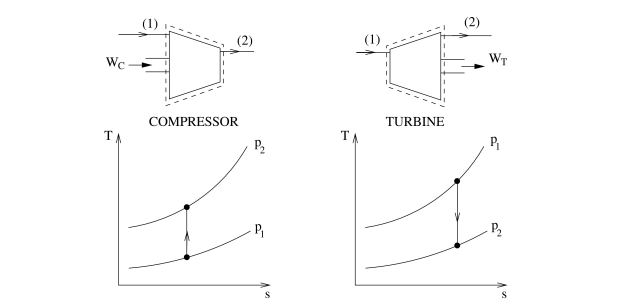
\includegraphics[width = 0.5\textwidth]{images/Screenshot 2024-04-03 212806.png}
    \caption{Compressor and turbine}
    \label{fig:enter-label}
\end{figure}

\newpage

\subsection{Gas turbines and jet engines}

In this final section, we will apply steady flow control volume analysis to study gas turbines and the simplest form of a jet engine. As with reciprocating internal combustion engines, a simplified air-standard cycle analysis will be adopted.

\begin{definition}[Gas turbine]
    A gas turbine is a device whose function is to produce shaft work in order to drive a generator, or a pump, or some other piece of rotating machinery.
\end{definition}

\begin{definition}[Jet engine]
    A jet engine is a device that produces no net shaft work - its function is to generate thrust by means of a high velocity exhaust jet.
\end{definition}

\subsubsection{The air-standard Joule cycle}

The main components of a typical industrial gas turbine are shown below.

\begin{figure}[h]
    \centering
    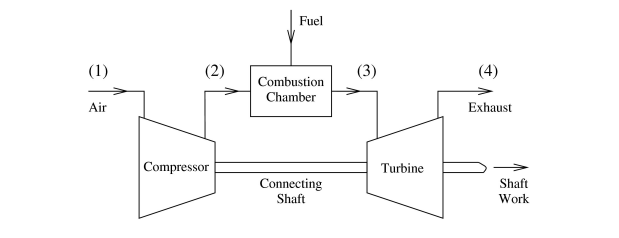
\includegraphics{images/Screenshot 2024-04-03 213414.png}
    \caption{Gas turbine}
    \label{fig:enter-label}
\end{figure}

Air is taken in at (1) and compressed at (2), at which its pressure is typically 12 - 40 times less than at (1). Fuel is then added and combustion occurs at more or less constant pressure. Hot, high pressure combustion gases then enter the turbine at (3) and expand down to the exhaust pressure at (4), which is usually the same as the ambient pressure $p$.

The gas turbine is clearly a flow device: there are two inflows (air and fuel) and one exit flow
(the exhaust). It would be quite possible to draw a control surface around the whole gas turbine
and then apply the steady-flow energy equation to compute the output shaft work. However, this requires accounting
for the enthalpy changes during combustion, a topic which has not yet been covered. Instead, we
consider the working fluid as air throughout and we model the combustion process as a constant
pressure heat input.

\begin{proposition}[The air-standard Joule cycle]
    The air-standard Joule cycle (sometimes called the Brayton cycle) is an approximate model of
the gas turbine that replaces the open-circuit “cycle” with a closed-circuit one, as shown below.
Note that each device (compressor, turbine, etc.) operates as a steady flow device so must be
analysed by the steady-flow energy equation (and not the First Law for a system). 
\end{proposition}

\begin{figure}[h]
    \centering
    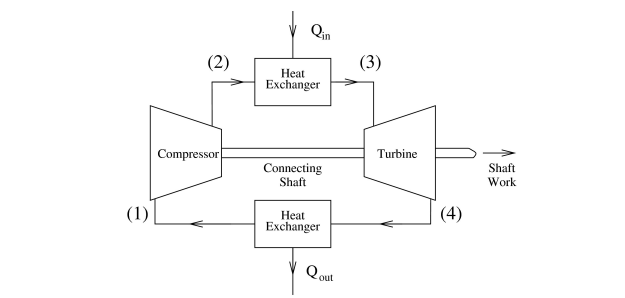
\includegraphics[width = 0.7\textwidth]{images/Screenshot 2024-04-03 213737.png}
    \caption{The Joule cycle}
    \label{fig:enter-label}
\end{figure}

The processes are as follows:

\begin{enumerate}
    \item (1) $\to$ (2): Isentropic compression
    \item (2) $\to$ (3): Constant pressure heat addition
    \item (3) $\to$ (4): Isentropic expansion
    \item (4) $\to$ (1): Constant pressure heat rejection
\end{enumerate}

\subsubsection{The jet engine}

The major components of the simplest form of the jet engine (a turbojet) are shown below.

\begin{figure}[h]
    \centering
    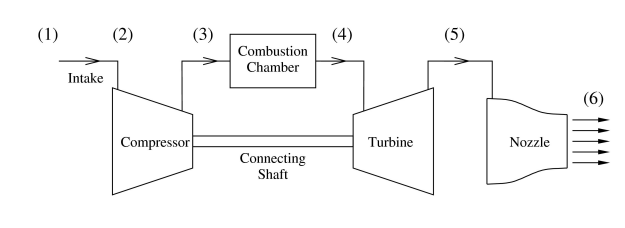
\includegraphics[width = 0.7\textwidth]{images/Screenshot 2024-04-03 214021.png}
    \caption{The turbojet engine}
    \label{fig:enter-label}
\end{figure}

The major difference between the jet engine and the gas turbine is that, rather than producing net shaft work, the turbine work output for a jet engine balances the compressor work input.

The processes for a jet engine are as follows:

\begin{enumerate}
    \item (1) $\to$ (2): Isentropic stagnation (intake)
    \item (2) $\to$ (3): Isentropic compression (compressor)
    \item (3) $\to$ (4): Constant pressure heat input (combustor)
    \item (4) $\to$ (5): Isentropic expansion (turbine)
    \item (5) $\to$ (6): Isentropic acceleration (nozzle)
\end{enumerate}

\begin{figure}[h]
    \centering
    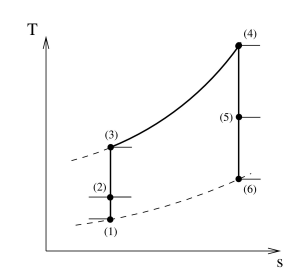
\includegraphics{images/Screenshot 2024-04-03 214437.png}
    \caption{The $T-S$ diagram for the turbojet}
    \label{fig:enter-label}
\end{figure}

It is not usually necessary to close the cycle with a fictitious process from (6) $\to$ (1), because we are normally interested in calculating the engine thrust, rather than efficiency. To do this, we simply apply the steady flow momentum equation for the whole engine.

\end{document}
